\section{DNN and CNN}
\subsection{Tensor notation}
\begin{definition}
A tensor $T$ of order $d$  is a multi-index array,
\begin{equation}
T \in \mathbb R^{n_1 \times n_2 \times \cdots \times n_d},
\end{equation}
with $i$-th dimension being $n_i$.
\end{definition}
\paragraph{Example 1: 2D grey image}
\begin{equation}\label{2DGreyImage}
T \in \mathbb{R}^{n_1 \times n_2}.
\end{equation}
\paragraph{Example 2: 2D color image}
\begin{equation}\label{2DColorImage}
T \in \mathbb{R}^{3 \times n_1 \times n_2}.
\end{equation}
\paragraph{Example 3: 3D grey image - MRI}
\begin{equation}\label{3DColorImage}
T \in \mathbb{R}^{ n_1 \times n_2 \times n_3}.
\end{equation}

\begin{definition}[Tensor Product]
If $X \in \mathbb R^{n_1 \times n_2 \times \cdots \times n_d}$ and $Y \in \mathbb R^{m_1 \times m_2 \times \cdots \times m_e}$, then the tensor product is noted as $\otimes$ with the next definition,
\begin{equation}
X \otimes Y \in \mathbb R^{n_1 \times n_2 \times \cdots \times n_d \times m_1 \times m_2 \times \cdots \times m_e},
\end{equation}
with
\begin{equation}
(X\otimes y)_{i_1, \cdots, i_d, j_1, \cdots,j_e} = X_{i_1, \cdots, i_d} Y_{j_1, \cdots, j_e}.
\end{equation}
\end{definition}
\paragraph{Example 5: Rank one matrix} If $x \in \mathbb{R}^n$ and $y \in \mathbb{R}^m$, then
\begin{equation}\label{3DColorImage}
x \otimes y \in \mathbb{R}^{n \times m},
\end{equation}
with
\begin{equation}
x \otimes y = x y^\top.
\end{equation}

\paragraph{Example 6: } If $X \in \mathbb{R}^{n_1\times n_2}$ and $Y \in \mathbb{R}^{m_1 \times m_2}$, then
\begin{equation}\label{3DColorImage}
X \otimes Y \in \mathbb{R}^{n_1 \times n_1 \times m_1 \times m_1},
\end{equation}
with
\begin{equation}
(X \otimes Y)_{i_1, i_2, j_1 ,j_2}  =  X_{i_1, i_2} Y_{j_1, j_2}.
\end{equation}

\begin{definition}[Tensor ``inner product"]
If
$$
X \in \mathbb R^{(n_1 \times n_2 \times \cdots \times n_d )\times
  (t_1\times t_2\times\cdots\times t_k)}
$$ and
$$
Y\in \mathbb R^{ (t_k\times t_{k-1}\times\cdots\times t_1)\times
  (m_1 \times m_2 \times \cdots \times m_e)},
$$
then the tensor ``inner product" with order $k$ is given by
\begin{equation}
X\odot_k Y \in \mathbb R^{n_1 \times n_2 \times \cdots \times n_d \times m_1 \times m_2 \times \cdots \times m_e},
\end{equation}
with
\begin{equation}
(X\odot_k Y)_{i_1, \cdots, i_d, j_1, \cdots,j_e}
=\sum_{s_1=1}^{t_1} \cdots\sum_{s_k=1}^{t_k}X_{i_1, \cdots, i_d, s_1,\cdots,s_k} Y_{s_k,\cdots,s_1,,j_1, \cdots, j_e}.
\end{equation}
\end{definition}
We note that
$$
X\otimes Y =X\odot_0Y
$$
For simplicity, we denote
\begin{equation}
X\cdot Y=X\odot_1Y \mbox{ and } X:Y=X\odot_2 Y  .
\end{equation}
\paragraph{Example 7: } If $x \in \mathbb{R}^{1\times n}$ and $y \in \mathbb{R}^{n}$, then
\begin{equation}\label{3DColorImage}
x \odot_1 y =xy= \sum_{i=1}^n x_{1,i} y_{i,1}.\in \mathbb{R}^{1}.
\end{equation}


\paragraph{Example 8: } If $X \in \mathbb{R}^{n_1 \times m}$ and $Y \in \mathbb{R}^{m \times n_2}$, then
\begin{equation}\label{3DColorImage}
X \odot_1 Y =XY\in \mathbb{R}^{n_1 \times n_2},
\end{equation}
with
\begin{equation}
(X \cdot Y)_{i,j} = \sum_{k=1}^m X_{i,k} Y_{k,j}.
\end{equation}
which is again the product of two matrices.

\begin{remark}
Without loss of generality, if the dimension and operation is clear, we note $\odot$ without $\odot_k$
\end{remark}

\newpage
\subsection{Single layer}
A singular layer linear neural network can be written as
$$
f(x, \theta)
=
\begin{pmatrix}
  f_1(x,\theta_1)\\
\vdots
\\
  f_m(x,\theta_m)
\end{pmatrix}
=
\begin{pmatrix}
 w_1 x+b_1, \\
\vdots
\\
 w_m x+b_m, \\
\end{pmatrix}
=
\begin{pmatrix}
 w_1\\
\vdots
\\
 w_m
\end{pmatrix}x
+
\begin{pmatrix}
b_1\\
\vdots
\\
b_m
\end{pmatrix}
=Wx+b=\theta \tilde x
$$
where
\begin{equation}
W\in \mathbb R^{m\times n},
\theta=(W,b)=
\begin{pmatrix}
  \theta_1\\
\vdots\\
\theta_m
\end{pmatrix}, \quad
\tilde x=
\begin{pmatrix}
  x\\
1
\end{pmatrix}
\end{equation}


We have
\begin{equation}
f(x; \theta )= W x+b, ~ \Theta = \{ \theta = (W,b) ~|~ W \in \mathbb{R}^{m \times n}, b \in \mathbb{R}^m \}.
\end{equation}

with $f: \mathbb{R}^n \to \mathbb{R}^m$.

\subsection{Deep neural networks (DNN)}
\begin{figure}[!ht]
\center{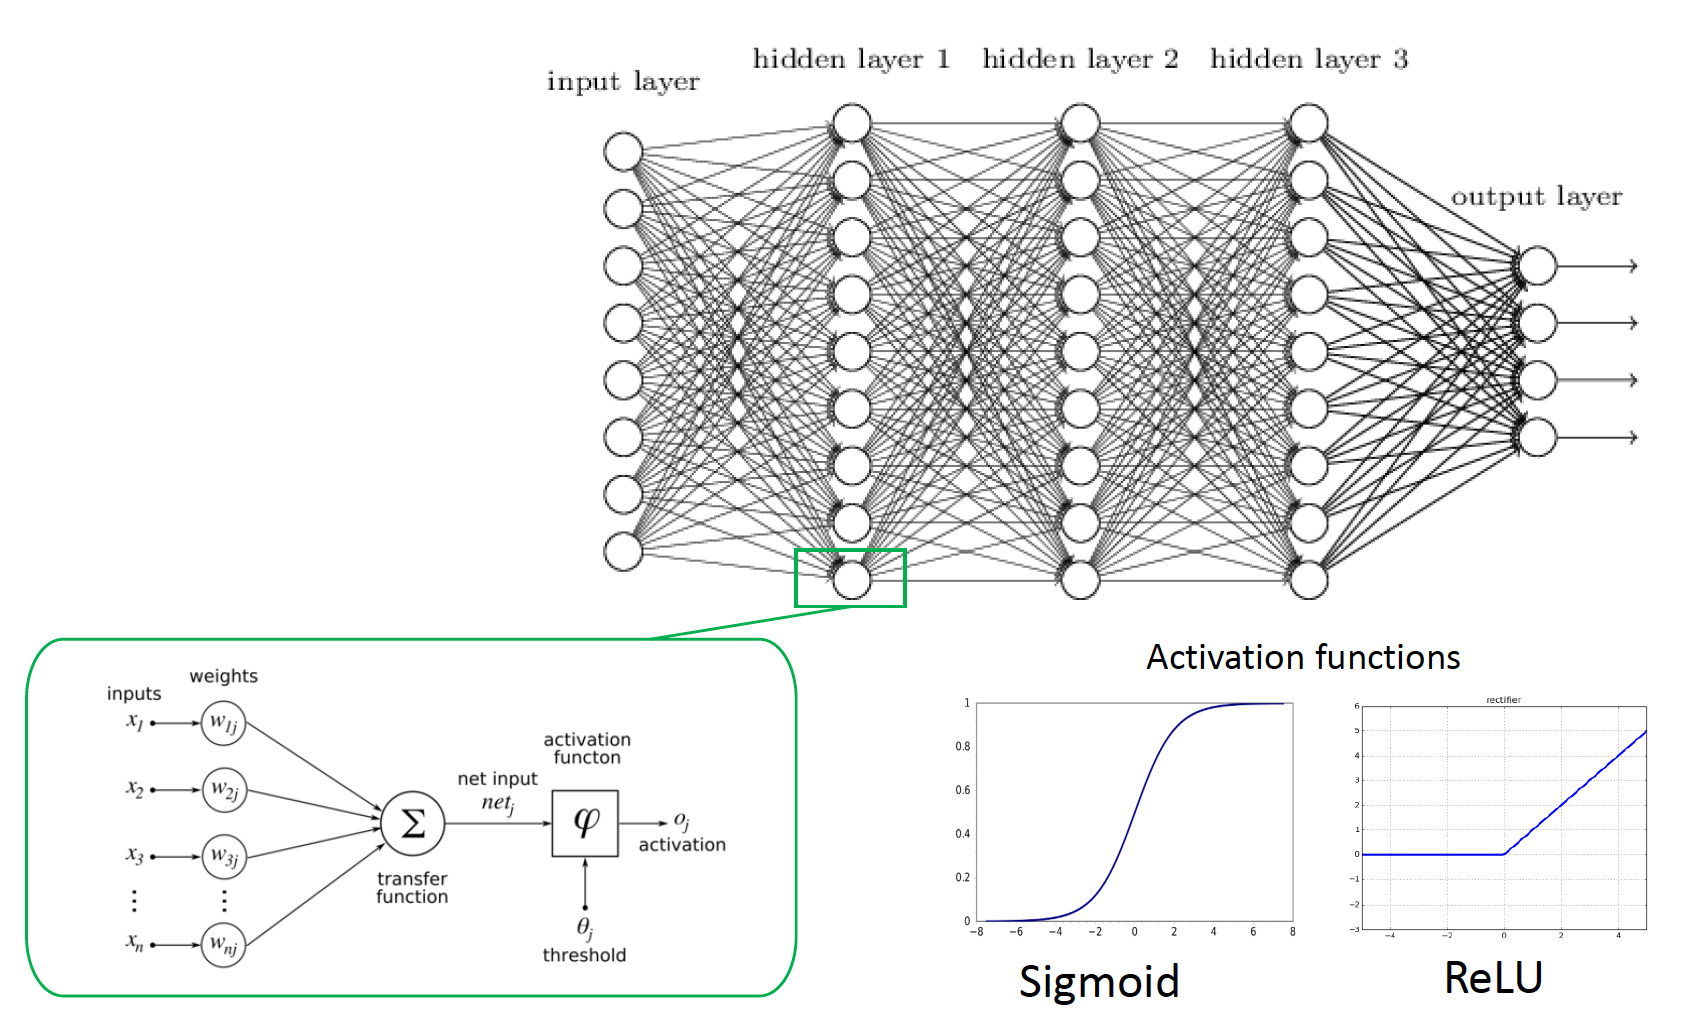
\includegraphics[width=12cm,height=6cm] {figures/ANN.png}}
\caption{A typical deep neural network}
\end{figure}
We consider a sequence of affine operations:
\begin{equation}
\theta^j: \mathbb R^{\hat{n}_{j}}\mapsto \mathbb R^{ n_{j}}.
\end{equation}
with
\begin{equation}\label{DNN_affinemap}
\theta^j(x) =  W^j x + b^j
=
(W^j, b^j)
\begin{pmatrix}
  x \\
1
\end{pmatrix}
=
\theta^j
\begin{pmatrix}
  x \\
1
\end{pmatrix}
\end{equation}
and
\begin{equation}
W^j\in \mathbb R^{n_j \times  \hat n_{j}}, b^j\in \mathbb R^{n_j}.
\end{equation}
With a slight abuse of notation, we also denote
\begin{equation}
\theta^j=(W^j, b^j)
=
\begin{pmatrix}
\theta^j_{1}\\
\vdots \\
\theta^j_{n_j}\\
\end{pmatrix}
\in \mathbb R^{n_j\times (\hat n_{j}+1)}.
\end{equation}

For $j=0$, we have the input data
$$
x\in \mathbb R^{\hat n_{0}}
$$
For MNIST data base, we have
$$
\hat n_0 = 784.
$$

We consider nonlinear activation function that is applied componentwise:
\begin{equation}\label{DNN_iteration_vector}
g:\mathbb R^{ n_{j-1}}\mapsto \mathbb R^{n_{j-1}},
\end{equation}
and polling functions
\begin{equation}\label{DNN_iteration_vector}
r^j:\mathbb R^{ n_{j-1}}\mapsto \mathbb R^{\hat n_{j}}.
\end{equation}
Poolling is not always applied after each application of activation.
When it is not applied, $r^j$ is identity and $\hat n_j=n_{j-1}$;   when
it is applied, $r_j$ is usually nonlinear and
$$
\hat n_j<n_{j-1}.
$$

We consider the pooled-activation functions:
\begin{equation}\label{DNN_iteration_vector}
g^j=r^j\circ g: \mathbb R^{{n}_{j-1}}\mapsto
\mathbb R^{\hat n_{j}}, \quad j =  1 :J.
\end{equation}
We note that
\begin{equation}
\theta^j\circ g^j:    \mathbb R^{{n}_{j-1}}\mapsto
\mathbb R^{n_{j}}
\end{equation}

We can then define a multi-layer neural network
	\begin{equation}\label{DNN_finallayer}
	f(x; \Theta) = f^J,
	\end{equation}
        with:
	\begin{equation}\label{DNN_iteration_vector}
	f^j(x,\Theta^j) = (\theta^j\circ g^j\circ
        f^{j-1})(x,\Theta^{j-1}), \quad j=1:J
	\end{equation}
where
\begin{equation}
\Theta^j=(\Theta^{j-1},\theta^j), \quad \Theta^0=\theta^0
\end{equation}
and
	\begin{equation}
	f^0(x)=\theta^0(x).
	\end{equation}

Here

\begin{align}
\Theta =\Theta_J =(\theta^0,\theta^1, \cdots, \theta^J)=( ({W^0}, {b^0}),({W^1}, {b^1}),
\cdots, ({W^J}, {b^J})) \\
\displaystyle
	\in  (\mathbb{R}^{n_0 \times (\hat n_0 + 1)}) \oplus \cdots
        \oplus  	(\mathbb{R}^{{n}_{J} \times (\hat
          n_{J}+1)})=
\oplus_{j=0}^J \mathbb{R}^{n_{j} \times (\hat n_{j} + 1)}
\end{align}




\subsection{Activation function}
        \begin{itemize}
	\item An general activation function(must be nonlinear) is
	$$g: \mathbb{R} \to  \mathbb{R}.$$
        \item The sigmoid function is
        $$\sigma(x) = \frac{1}{1 + e^{-x}}.$$
	\item The ReLU(rectified linear unit) is
	$$
	ReLU(x) = r(x) = \max(0, x).
	$$
	\item The Heaviside function is
	$$
	H(x ) = \begin{cases}
	0 \quad &\text{if} ~ x \le 0, \\
	1 \quad &\text{if} ~ x > 0.
	\end{cases}
	$$
	\item The new activation function as ReLU1 is:
	$$
	\tau(x) = r(x) - r(x-1) = \begin{cases}
	0 \quad &\text{if} ~ x \le 0, \\
	x \quad &\text{if} ~  0 < x \le 1, \\
	1  \quad &\text{if} ~ x > 1.
	\end{cases}
	$$

	\end{itemize}

\subsection{Classification properties under this notation}
\begin{theorem}
  If $\{A_k\}_{k=1}^c$ are separable with positive distance, then it
  can be separated by $f(x; \Theta) = f^2$, with $W^2= id, b^2=0$ and
  all activation function is $\tau$.
\end{theorem}

\subsection{CNN for images}
\subsection{General setup}
\begin{enumerate}
\item Data:
	\begin{itemize}
	\item Input set: $\bm{X} = \{x_1, \cdots, x_N\}$
	\item Output set: $\bm{y} =  \{y_1, \cdots, y_N\}$
	\item Generally,  input use $x \in \mathbb{R}^{\hat c_0 \times \hat n_1\times \cdots \times \hat n_d }$, with a label $y \in \mathbb{R}^c$ (output for classification problem)
	\item Here $\hat c_0$ means the channel dimension and $\hat n_1\times \cdots \times \hat n_d$ means the essential dimension.
	\end{itemize}
      \item Here we use $x \in \mathbb{R}^{\hat c_0 \times n \times n} $,
        $y \in \mathbb{R}^c$ as example.
\item Kernels: in CNN they generally use $K^i$ and $b^i$ to stand for the kernels and bias.
\end{enumerate}

\paragraph{Example 1: 2D grey image}
\begin{equation}\label{2DGreyImage}
c_0=1, d=2
\end{equation}
\paragraph{Example 2: 2D color image}
\begin{equation}\label{2DColorImage}
c_0=3, d=2
\end{equation}
\paragraph{Example 3: 3D grey image - MRI}
\begin{equation}\label{2DColorImage}
c_0=1, d=3
\end{equation}


\subsection{DNN for images under tensor notation}

 Multilayer structures in convolutional layers is totally the same for \eqref{DNN_affinemap} - \eqref{DNN_finallayer}: the only difference  is the structure of affine map:

\begin{equation}\label{CNN_affinemap}
\theta^j_{p}(x) =  W^j_p \odot_3 x + b^j_p \in \mathbb R^{n_j \times n_j}, \quad p=1:c_j
\end{equation}

\begin{equation}\label{CNN_affinemap}
\theta^j(x) =  W^j\odot_3 x + b^j
\end{equation}
with
\begin{equation}
\theta^j: \mathbb R^{\hat c_j  \times \hat{n}_{j} \times \hat n_{j} } \mapsto \mathbb{R}^{c_j \times n_{j} \times n_j }.
\end{equation}

Here
\begin{equation}
W^j \in \mathbb{R}^{(c_j \times n_{j} \times n_j) \times
  (\hat{n}_{j} \times \hat n_{j}\times \hat c_{j} )}, \quad
b^j\in  \mathbb R^{c_j \times n_{j} \times n_j},
\end{equation}
and
\begin{align}
\theta^j  &= \{W^j , b^j\}  \in \mathbb{R}^{(c_j \times n_{j} \times n_j) \times
  (\hat{n}_{j} \times \hat n_{j}\times \hat c_{j} )} \oplus \mathbb R^{c_j \times n_{j} \times n_j} \\
  &\cong  \mathbb{R}^{(c_j \times n_{j} \times n_j) \times
  (\hat{n}_{j} \times \hat n_{j}\times c_{j} + 1 )}
\end{align}

We note that
\begin{equation}
\hat n_0 =n  .
\end{equation}

We consider nonlinear activation function applied element wise:
\begin{equation}\label{CNN_iteration_vector}
g: \mathbb R^{c_{j-1} \times n_{j-1} \times n_{j-1} }\mapsto  \mathbb R^{c_{j-1} \times n_{j-1} \times n_{j-1}},
\end{equation}
and polling functions
\begin{equation}\label{CNN_iteration_vector}
r^j: \mathbb R^{c_{j-1} \times n_{j-1} \times n_{j-1} }\mapsto  \mathbb R^{\hat c_j \times \hat n_{j} \times\hat n_j }.
\end{equation}

We also consider ``pooled-activation'' functions:
\begin{equation}\label{CNN_iteration_vector}
g^j=r^j\circ g:  \mathbb R^{c_{j-1} \times n_{j-1} \times n_{j-1} }\mapsto
\mathbb  \mathbb R^{\hat c_j \times \hat n_{j} \times \hat n_j }, \quad j  = 1:J.
\end{equation}



We have the multi-layer DNN structure like:
	\begin{equation}\label{CNN_iteration_vector}
	f^j(x,\Theta^j) = (\theta^j\circ g^{j}\circ f^{j-1})(x,\Theta^{j-1}) \in \mathbb{R}^{c_j \times n_j \times n_j }
	\end{equation}
where
\begin{equation}
\Theta^j=(\Theta^{j-1},\theta^j), \quad \Theta^0=\theta^0
\end{equation}
	with
	\begin{equation}
	f^0(x)=\theta^0(x).
	\end{equation}

At last, we get
	\begin{equation}\label{CNN_finallayer}
	f(x; \Theta) = f^J.
	\end{equation}

        Roughly speaking, \eqref{CNN_affinemap} -
        \eqref{CNN_finallayer} is totally the same for \eqref{DNN_affinemap}
        - \eqref{DNN_finallayer} in tensor notation.

\subsection{CNN for image}
A convolution operation is a special linear mapping of the following form:
\begin{equation}
\theta^j(x) = K^j \circledast x + {\rm{diag}(b^j)} \cdot \bm{1}_{c_j \times n_j \times n_j} \quad
\in\mathbb R^{c_j\times n_j\times n_j}.
\end{equation}
with
	\begin{equation}
	K^j \in \mathbb{R}^{ c_{j} \times \hat c_{j} \times (2k+1) \times (2k+1)},  \quad \text{and} \quad b^j \in \mathbb{R}^{c_j},
	\end{equation}
	and
	\begin{equation}
	\bm{1}_{c_j \times n_j \times n_j} = 1_{c_{j}} \otimes 1_{n_j} \otimes 1_{n_j}
	\end{equation}
for $k = 0, 1, 2, 3...$.

Give $p\in \{1,\ldots c_j\}$
\begin{equation}
(\theta^j(x))_p= (K^j \circledast x)_p+b^j_p{\bm 1}_{n_j\times n_j}
\end{equation}
and
\begin{equation}
 (K^j \circledast x)_p
= \sum_{q=1}^{\hat c_{j}} K^{j}_{p,q} \ast x_q \in \mathbb{R}^{n_j \times n_j}, \quad p= 1:c_j.
\end{equation}
where
$$
K^{j}_{p,q}\in \mathbb R^{(2k+1)\times (2k+1)}, x_q\in \mathbb
R^{\hat n_{j}\times \hat n_{j}}.
$$
Here $\ast$ is the traditional convolution defined as:
\begin{equation}\label{ConvPadding}
(K \ast x)_{i,j} :=\sum_{s, t = -k}^k  K_{s+k+1,t+k+1} x_{i + s, j + t},
\end{equation}
Here we assume implicitly that a special ``padding'' is used such that
\begin{equation}
  \label{zero-padding}
x_{i,j}=0 \mbox{ if } i, j\le 0 \mbox{ or } i, j > n_j.
\end{equation}


\subsection{CNN with stride for image}
\subsubsection{Polling and stride}
If we use stride $s$, we have have the stander convolution operator with stride $s$ as:
\begin{equation}\label{equ:convstride}
(K\ast_{s} x)_{i,j} = \sum_{p, q = -k}^k K_{p+k+1,q+k+1}x_{is + p, js + q} .
\end{equation}
This stride properties in some application are often used as pooling(subsampling, coarsening).

Here we can define a special pooling operator as $S(\cdot,s)$ which likes the $C/F$ split for choosing coarse point:
\begin{equation}
S(X,s)_{i,j} = X_{is, js },
\end{equation}
then we have:
\begin{equation}\label{equ:stride}
X \ast_s K = S(X\ast K, s),
\end{equation}
with the $\ast$ and $\ast_s$ defined by \eqref{ConvPadding} and \eqref{equ:convstride}
\begin{proof}
\begin{align}
S(X \ast K,s)_{i,j} &= (X \ast K)_{is, js}  \\
&= \sum_{p, q = -k}^k K_{p+k+1,q+k+1}x_{is + p, js + q}  \\
&= (X \ast_s K)_{i,j}.
\end{align}
\end{proof}


We note convolution with stride as:
\begin{equation}
\theta^j: \mathbb R^{\hat c_j \times \hat{n}_{j} \times \hat n_{j} } \mapsto \mathbb{R}^{c_j \times n_{j} \times n_j }.
\end{equation}
with
\begin{equation}
\theta^j(x) = K^j \circledast_{s^j} x + {\rm{diag}(b^j)} \cdot \bm{1}_{c_j \times n_j \times n_j} \quad
\in\mathbb R^{c_j\times n_j\times n_j}.
\end{equation}
with
	\begin{equation}
	K^j \in \mathbb{R}^{ c_{j} \times \hat c_{j} \times (2k+1) \times (2k+1)},  \quad \text{and} \quad b^j \in \mathbb{R}^{c_j},
	\end{equation}
	and
	\begin{equation}
	\bm{1}_{c_j \times n_j \times n_j} = 1_{c_{j}} \otimes 1_{n_j} \otimes 1_{n_j}
	\end{equation}
for $k = 0, 1, 2, 3...$.

Give $p\in \{1,\ldots c_j\}$
\begin{equation}
(\theta^j(x))_p= (K^j \circledast_{s^j} x)_p+b^j_p{\bm 1}_{n_j\times n_j}
\end{equation}
and
\begin{equation}
 (K^j \circledast_{s^j} x)_p
= \sum_{q=1}^{\hat c_{j}} K^{j}_{p,q} \ast_{s^j} x_q \in \mathbb{R}^{n_j \times n_j}, \quad p= 1:c_j.
\end{equation}
where
$$
K^{j}_{p,q}\in \mathbb R^{(2k+1)\times (2k+1)}, x_q\in \mathbb
R^{\hat n_{j}\times \hat n_{j}}.
$$
Here $\ast_{s^j}$ is the stander convolution with stride as definition before.
